  \chapter{The High Resolution Spectrometer Optimization $\simeq 30$}

PRex-II Experiment was operated on Jefferson Lab High-Resolution Spectrometer(JLab). The kinematics of the scattered electrons have to be measured on the Vertical Drift Chambers which are installed after the magnetic chains. All the measurements have to be converted back to the target coordination system in order to get the result. This chapter will discuss the detail of JLab HRS calibration, the calculation of the 4-momentum transfer square, and the GEM detector analysis. 


\section{High-Resolution Spectrometer Optics Calibration}

(a more detailed apparatus could/will be found in another chapter describing the detailed experiment configuration)

The Vertical Drift Chamber provides the HRS spatial resolution capability. Each of the two HRS spectrometers contains two Vertical Drift Chamber(VDC). each chamber has 750 wires in two (U, V) planes, position resolution of 100 um per plane. Four VDC chamber layers of wires can provide partial spatial location $x$, $y$ together with particle angle $\theta$ and $\phi$. The kinematics, like scattered angle and scattered momentum, need to derive from the four direct measurable parameters(VDC $x$, $y$,$\theta$,$\phi$). The calibration procedure can be categorized into three steps:

\begin{itemize}
    \item VDC drift time $t_0$ calibration
    \item VDC geometry constant calibration 
    \item spatial and angular calibration
    \item momentum calibration
\end{itemize}

Vertical Drift Chamber measures the spatial position by measuring the particle drift time. $t_0$ serves as the starting time of the VDC counter. Carefully calibrated $t_0$ is critical to the spatial and angular resolution of the VDC. To simplify the regression model and easily converge, the spatial, angular, and momentum parameters are calibrated from the focal plane. The VDC geometry constants are used to convert the direct measurements on the VDC plane to the focal plane. Before going into the detail of the calibration, here first introduce the coordination system used in the following contest. 

\subsection{coordinate system}


To simplify the calculation, couples of different coordinate systems are used. In this section, five coordinate systems and their directive relations are briefly introduced. A more detailed coordinate system of Jefferson Lab Hall A can be found in the ESPACE User Manual\cite{espace2002manual}.  

\subsubsection{Hall Coordinate System}
The center of the Hall Coordinate system is defined as the intersection of the electron beam and the vertical symmetry axis of the target system. $z$ is along the beam dump direction. $y$-axis is pointing vertically up against gravity.

[add HCS coordination plot]

\subsubsection{Target Coordinate System}

Each High-Resolution Spectrometer(HRS) has its own target coordinate system. Ideally, the center of the target coordinate system coincides with the center of the Hall A coordinate system. The distance from the hall A center to the midpoint of the center of the sieve slit hole is defined as $Z_0$ ($Z^{HRSE}_0 = 1.181 m$, $Z^{HRSH}_0 = 1.178 m$). The center of the target coordinate system is defined as $Z_0$ distance from the sieve slit(ref to chapter xx section xx) with $z$-axis perpendicular to the center of the sieve slit plane pointing to the beam direction. The $x$-axis is parallel to the sieve slit surface with $x$ pointing vertically down. The $\theta$ and $\phi$ angle is defined as $\frac{dx_{tg}}{Z_0}$ and $\frac{dy_{tg}}{Z_0}$ respectively.

[add TCS plot]


\subsubsection{Detector Coordinate System}

Each of the VDC chambers has 368 wires placed at $\pm 45 ^{\circ} u/v$ direction. The center of the detector coordinate system is defined as the intersection of wire 184 of the VDC1 U1 plane and the perpendicular projection of wire 184 in the VDC1 V1 plane onto the VDC1 U1 plane. $x$-axis is along the long edge of the VDC plane, while y is along the short edge of the VDC plane and $z$ is perpendicular to the VDC plane and pointing upwards. 

Let's take $p_{vdc,n}$ (where ${n=1-4}$)to be the cross position of a particle with each VDC plane. The vertex can be calculated with the following equation. 

\begin{equation}
    \tan \eta_{1} = \frac{p_{vdc,3} - p_{vdc, 1}}{d1}    
\end{equation}
\begin{equation}
    \tan \eta_{2} = \frac{p_{vdc,4} - p_{vdc, 2}}{d1}    
\end{equation}

For ideal experimental configurations, we take the following assumptions:
\begin{enumerate}
    \item All the VDC wires are positioned on a 2D VDC plane
    \item All the VDC wires are oriented in $45\circ$ angle
    \item there is no distortion with the VDC wires
    \item all the VDC frames a perfect parallel to each other 
    \item the center of each VDC plane is known with no error
\end{enumerate}

Given the above assumption, The trajectory position and vertex angles in the detector plane coordinate system can be derived with the following equation 

\begin{equation}
    \theta_{det} = 
\end{equation}
    
\begin{equation}
    \phi_{det} = 
\end{equation}

\begin{equation}
    x_{det} =
\end{equation}

\begin{equation}
    y_{det} =
\end{equation}

Even though the VDC could not be ideal, the distortions would be very small and through HRS Optics, those un-idea errors could be corrected. 

In Hall A analyzer, the VDC result will be given in the detector plane coordinate system.

[add vdc, DCS plot]

\subsubsection{Transport Rotation Coordinate System at the focal plane}
The transport coordinate system at the focal plane is defined as rotating the detector coordinate system by $45^{\circ}$ along the y-axis. Ideally the z-axis along the central beam ray. 

Given the particle position at the detector coordinate system, the transport rotation coordinate system can be derived as:

\begin{equation}
    \theta_{tra}  = 
\end{equation}

\begin{equation}
    \phi_{tra} =
\end{equation}

\begin{equation}
    x_{tra} =
\end{equation}

\begin{equation}
    y_{tra} = 
\end{equation}


[optimization the TRCS ??]


[add the plot of the transport coordinate system plot]


\subsubsection{Focal plane Coordinate System}

The focal plane coordinate system used for HRS analysis is a rotated coordinate system, obtained by rotating the Detector Coordinate System (DCS) around its y-axis by an angle. This angle is determined by the angle between the local central ray and the z-axis of the DCS, and as a result, the z-axis of the Focal Plane Coordinate System (FCS) rotates as a function of the relative momentum p.

To ensure easy convergence, the HRS Optics Tensor is calibrated with respect to the angles $\theta$ and $\phi$, the vertical position $y$, and the relative momentum $dp$ on the Focal Plane Coordinate System.

\begin{equation}
    x_fp = x_{tra}    
\end{equation}

\begin{equation}
    y_{fp} = y_{tra} - \sum y_{i000}x^i_{fp}  
\end{equation}

\begin{equation}
\theta_{fp} = \frac{\theta_{det} + \tan\rho}{1 - \theta_{det}\tan\rho}
\end{equation}


\begin{equation}
    \phi_{fp} = \frac{\phi_{det} - \sum p_{i000}x^i_{fp}}{cos \rho - \theta_{det} sin\rho}
\end{equation}

here  in the equation:

\begin{equation}
    \tan\rho  = \sum t_{i000}x^i_{fp}
\end{equation}


the code used for calibration of the focal plane constant can be found on this GitHub repository: https://github.com/Jiansiyu/GeneralScripts/blob/master/vdcConstantOpt

[need to add the derivation of the above equations]

[need to add the Focal plane coordination system plot]

\subsection{the calculation of the coordinate system (merge with the prev sub-section?)}

\subsubsection{correction the initial drift time}
Each HRS spectrometer is equipped with a package of four Vertical Drift Chambers (VDCs) that are oriented in the UV direction. The VDCs are filled with Argon (Ar) and flammable ethane, which is bubbled through alcohol. The gas filling is routed and delivered using the Hall A Gas System. Each wire in the VDCs is connected to a 3.5 kV high-voltage source.

When a charged particle passes through the VDC chamber, it ionizes the gas atoms, creating a trail of ionized electrons along its path. The ionized electrons drift along the electric field lines due to the high voltage between the high voltage plane and signal wires. This ionization produces a pulse on the signal wires. Each VDC chamber contains 368 wires, and each wire is connected to a pre-amplifier. The amplified pulse signal is then passed through a discriminator and used to trigger the Time-Digital Converter (TDC). The TDC is stopped by the Hall overall event trigger.

After the particle trespass into the chamber, normally it will fire a cluster that contains 4-6 wires. As shown in Fig \ref{fig:vdc_wire_ionization_cluster}, the cross point between the trajectory of the particle and the VDC plane could be measured by measuring the drift distance between each wire. The drift distance is measured with the drift time that gets from the Time-Digital-converter. An accurate start time would be critical to get an accurate drift distance to get an accurate position on VDC.  If the threshold is set too high or too low, the VDC drift distance would be biased. An example of an improper setting of $T_0$ is shown in the plot, where a large number of 'wire shadows' can be observed. These shadows are caused by measurement bias.

\begin{figure}
    \centering
    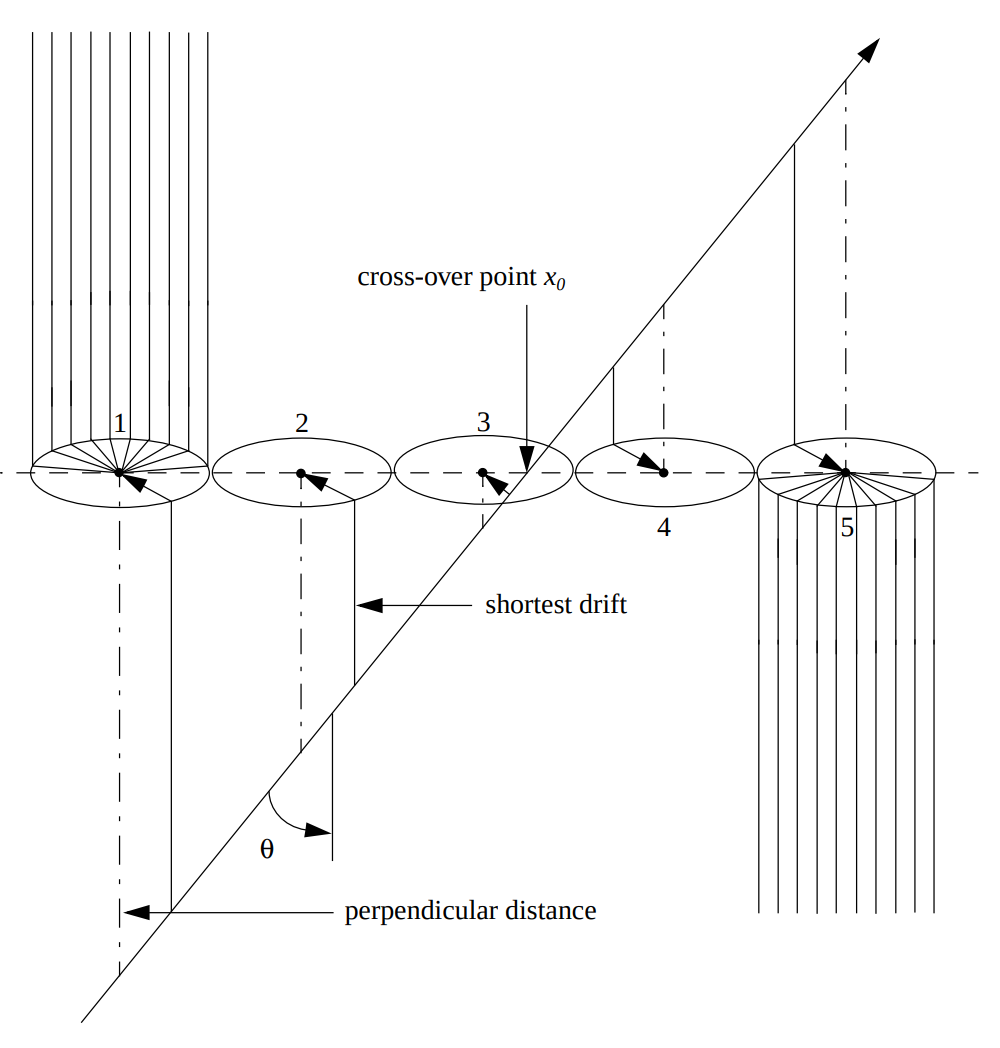
\includegraphics[scale = 0.25]{images/chap3/vdc_wire_ionize.png}
    \caption{Vertical Drift Chamber Ionization (need to redraw)}
    \label{fig:vdc_wire_ionization_cluster}
\end{figure}

\begin{figure}
    \centering
    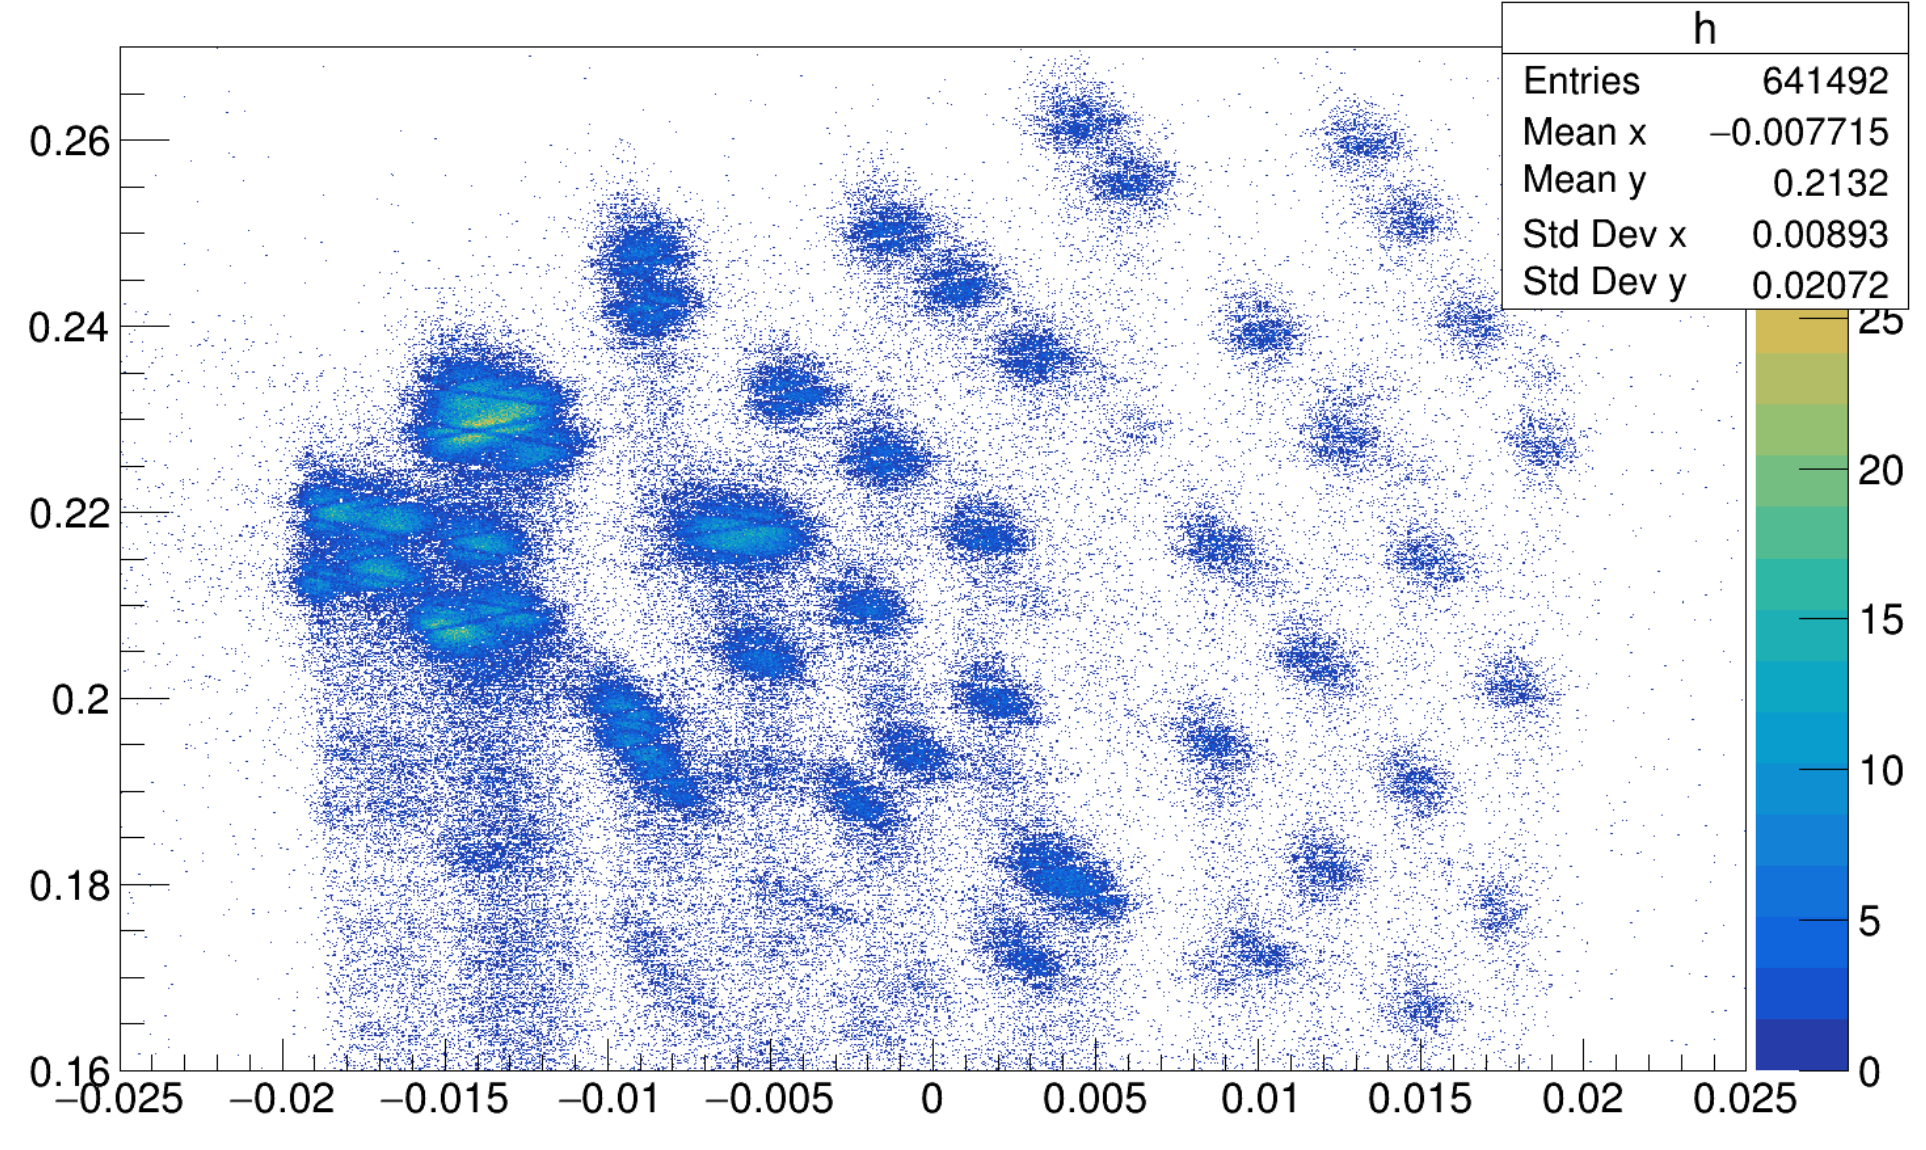
\includegraphics[width=\textwidth]{images/chap3/vdc_t0_before_correction.png}
    \caption{vdc $x$ vs $y$ on vdc detector plane before T_0 correction}
    \label{fig:vdc_t0_before_correction}
\end{figure}


\begin{figure}
    \centering
    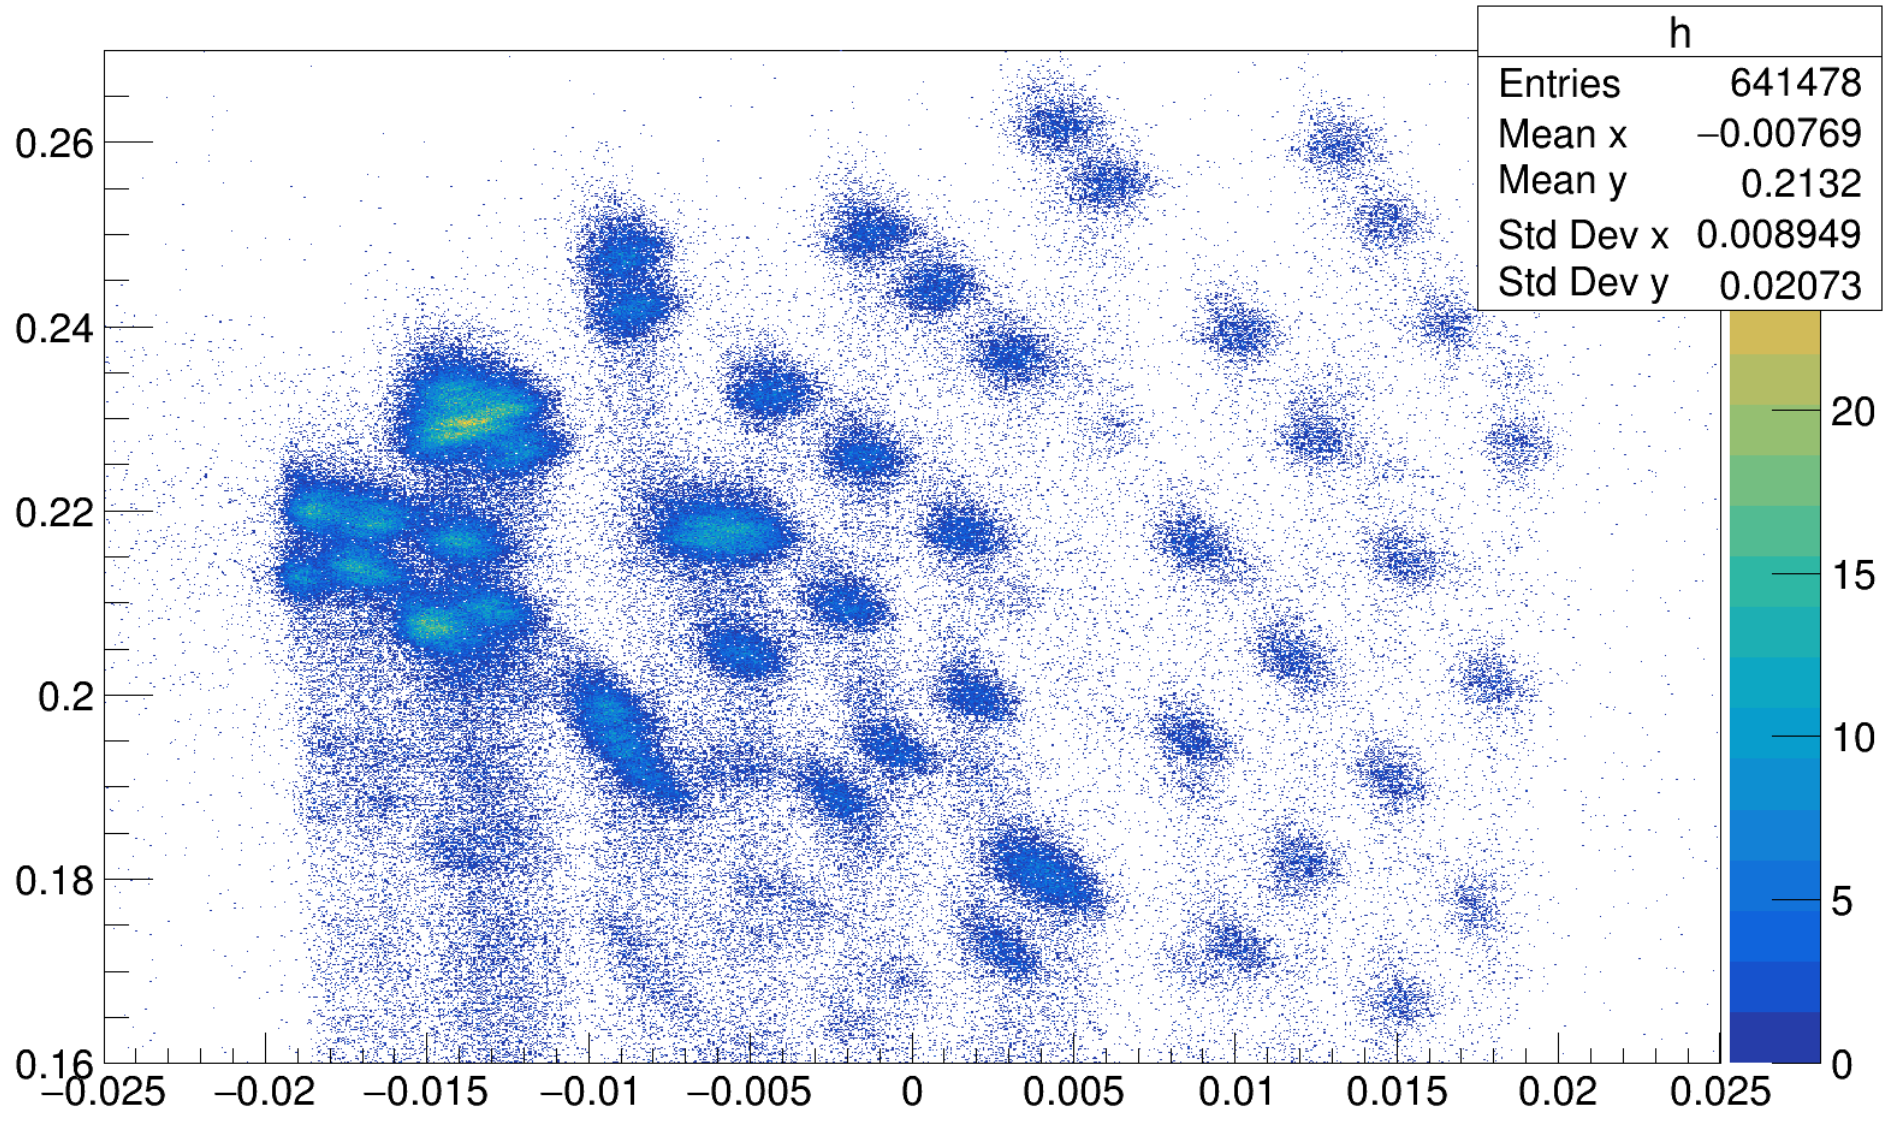
\includegraphics[width=\textwidth]{images/chap3/vdc_t0_after_correction.png}
    \caption{vdc $x$ vs $y$ on vdc detector plane after T_0 correction}
    \label{fig:vdc_t0_after_correction}
\end{figure}

The $t_0$ could be calibrated by adjusting the time offset of each TDC channel. In order to calibrate the TDC for all the VDC range, the data should be white spectrum runs that covers all focal plane range with high statistics. 

Here is a procedure of calibration of the TDC $T_0$: [need to check again.]
\begin{enumerate}
    \item Fit the failing tail of the spectrum. 
    \item take the 1.4 $\sigma$ before the peak time
\end{enumerate}



\subsubsection{convert to the transport coordinate system}
As it definition says. The focal plane should pass (0,0) for central beam runs. 

\subsubsection{convert to the focal plane coordinate system}

[check the sides] 


\subsubsection{feature engineering}
\subsubsection{feature selection}
% \lipsum[1-20]
\subsection{Apparatus[deprecated]}

Move to a separate chapter describing the apparatus and experiment details

\begin{itemize}
    \item Overview of the HRS structure
    \item septum magnet 
    \item Vertical drift chamber 
    \item GEM detector
    \item supporting equipment used for optimization only sieve slide

    \item coordination system of the Jefferson Lab Hall A
    \item coordination system of the HRS
\end{itemize}


\subsection{HRS model}

\begin{itemize}
    \item mathematical model of the HRS
    \item constant parameter optimization
    \item Vertical Drift Chamber time optimization
    \item carbon calibration(dashed lines in the VDC spectrometer)
    \item math why higher order contribute, a discussion notes
    \item feature selection techniques
    \item linear regression
    \item result validation
    \item result and discussion
\end{itemize}
\subsubsection{supervised linear regression}
\subsubsection{feature selection technics}
\subsubsection{mathematics about the linear regression, LASSO and ridge regression}

\subsection{VDC geo-constant calibration}
\subsection{Raster calibration}

% \subsubsection{Linear Regression and mathematics approximation}




% \subsection{}section{feature selection}

% \subsubsection{general consideration in regression}

% \subsubsection{features in regression}

% \subsubsection{LASSO feature reduction regression}

% \subsubsection{ridge feature reduction regression}

% \subsection{autoML and more}

% \section{Momentum optimization}

% \section{Regression Result validation}

% \subsection{carbon result check}

% \subsubsection{first, second, third momentum check}

% \section{momentum reconstruction}

% \section{scattered angle reconstruction and correction}

% \section{a second thought/attempt on the regression}

% \subsection{another more complicated model}